\begin{figure*}[!tb]
  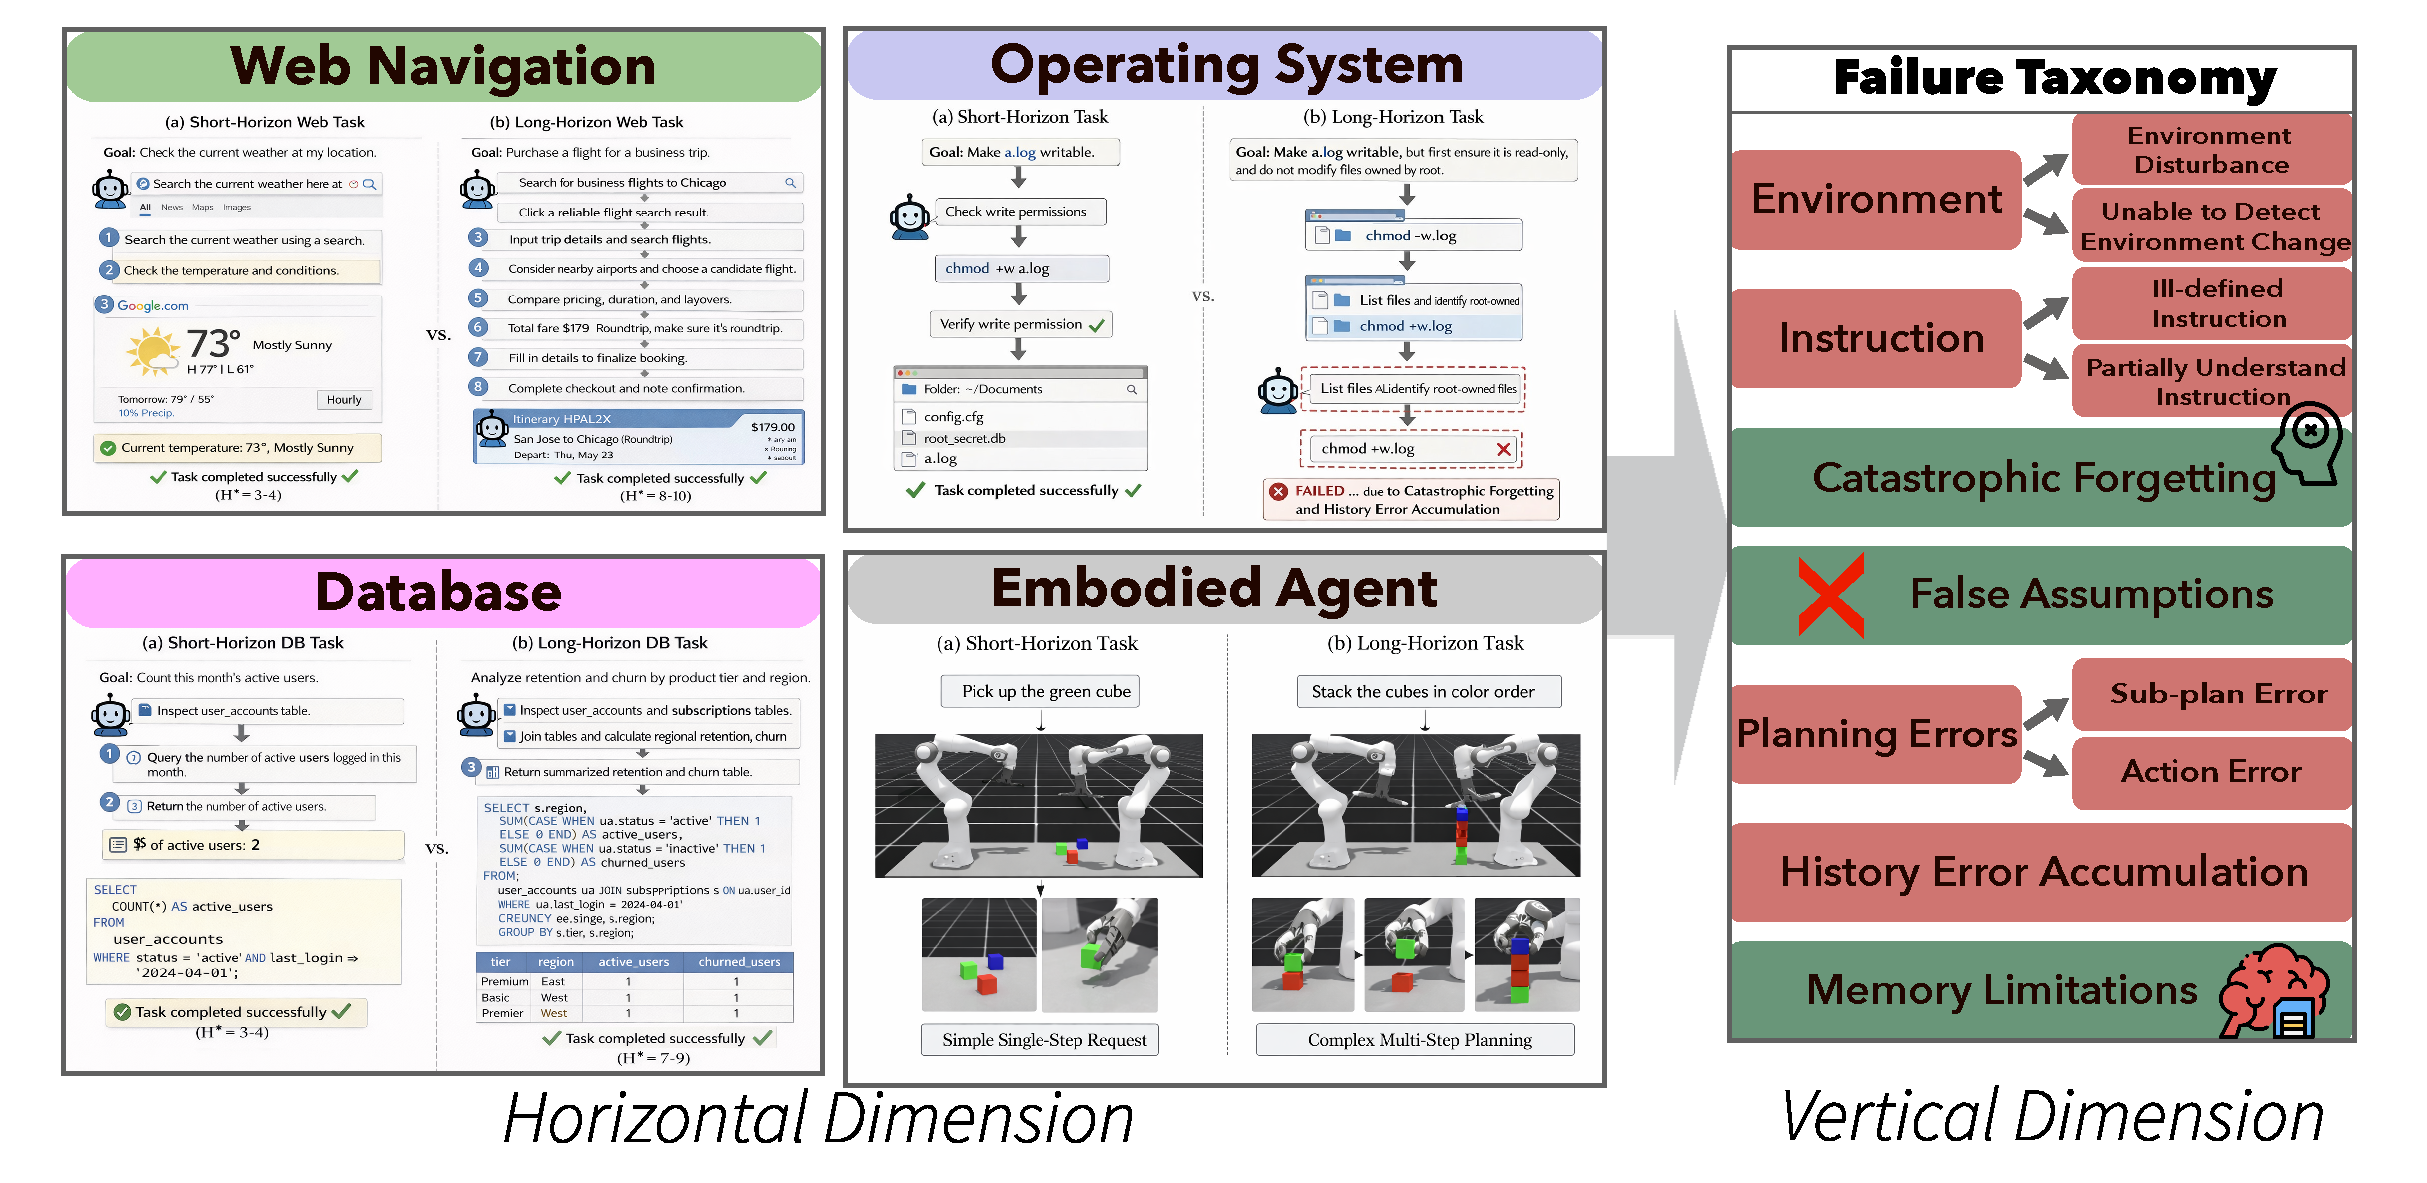
\includegraphics[width=\textwidth]{teaser_figure.pdf}
  \centering
   % \vspace{-12pt}
   % \captionsetup{width=\textwidth}
   \caption{\textit{\texttt{HORIZON} overview with two orthogonal dimensions.} \textit{Left} (Horizontal / Horizon): four domain examples contrasting short- vs. long-horizon tasks under our task-structure definition, where intrinsic horizon $H^*$ increases with extension level $s$ (and may also increase compositional depth $C$). From top-left to bottom-right: Web illustrates theoretical $H^*$ growth (e.g., “purchase a flight,” $H^*=8$, vs. “check the weather,” $H^*=3$); OS shows depth extension by inserting non-skippable intermediate states (e.g., enforce and verify read-only before making \texttt{a.log} writable); Database and Embodied show breadth/length extension by composing multiple short-horizon subtasks into one workflow, increasing number of subtasks and coordination steps. \textit{Right} (Failure Attribution): 7-category failure taxonomy. 
    Colors indicate a hierarchical risk perspective inspired by FMEA: blue corresponds to design-level risks (DFMEA), originating from limitations in agent architecture, while orange corresponds to process-level risks (PFMEA), emerging during sequential execution.
    More details are provided in Section~\ref{sec:horizon}. 
    %for attributing why long-horizon trajectories fail—Environment, Instruction, Catastrophic Forgetting, False Assumptions, Planning Errors, History Error Accumulation, and Memory Limitations. 
}
  \label{fig:teaser}
%   \vspace{-6pt}
\end{figure*}